\chapter{Odbiornik}


Centralną częścią prezentowanego prototypu jest odbiornik,
jego zadaniem jest wysyłanie sygnałów sterujących do nadajnika, zbieranie ultradźwięków z otoczenia oraz przesłanie
ich do dalszej analizy do komputera.
Składa się on z sześciu części (rysunek \ref{fig:odbiornik_szkic}):

\begin{itemize}
 \item trzech modułów ultradźwiękowych przetwarzających ultradźwięki na sygnał elektryczny
 \item płytki prototypowej \textit{stm32f4-discovery} \cite{bib:stm32f4Discovery}, która odpowiada za komunikację z komputerem
 \item przystawki do \textit{stm32f4-discovery} przystosowującej sygnały elektryczne z modułów ultradźwiękowych
  do poziomów akceptowalnych przez \textit{stm32f4-discovery}
 \item ramy, na której umieszczone są moduły ultradźwiękowe
\end{itemize}


\rysunek{odbiornik_szkic}{szkic odbiornika}{\label{fig:odbiornik_szkic}}


\section{Budowa i zasada działania}

Głównym elementem odbiornika stanowi płytka prototypowa \textit{stm32f4-discovery} \cite{bib:stm32f4Discovery},
jej zadaniem jest umożliwienie komunikacji pozostałych komponentów z komputerem.
\textit{Stm32f4-discovery} oparty jest o ARMowy procesor STM32F407VGT6 \cite{bib:stm32f407}, posiada on wbudowane trzy 12 bitowe przetworniki
analogowo-cyfrowe umożliwiające samplowanie z prędkością dochodzącą do 2.4MSPS, które wykorzystane zostały do próbkowania
sygnałów pochodzących z modułów ultradźwiękowych. Procesor umożliwia również komunikację z komputerem poprzez 
port USB z prędkością 12MB/s.

Oprogramowanie płytki prototypowej oparte jest na bibliotece \textit{stm32 usb 101} \cite{bib:stm32_usb_101}
zapewniającej komunikację z komputerem, do której dodana została obsługa przetworników ADC.
Program poprzez port USB dostaje komunikat, który z czterech nadajników ma nadawać, ta informacja przekazywana jest
dalej do nadajnika w raz z sygnałem wyzwalającym, następnie uruchamiane są trzy przetworniki ADC, które 
samplują odbierany dźwięk i poprzez DMA zapisują trzy kanały w pamięci procesora.
Częstotliwość pracy przetworników ustawiona jest na 1.6MSPS co daje średnio 40 sampli na jedną sinusoidę nadanego 40kHz sygnału.
Program zapamiętuje 16kS na każdym kanale, co przy prędkości dźwięku 340m/s daje maksymalną mierzoną odległość rzędu 3.5 metrów.
Po zebraniu w sumie 48kS, całość przesyłana jest do komputera w celu dalszej analizy.
Cały proces powtarzany jest dla każdego z czterech przetworników piezoelektrycznych nadajnika, 
co w sumie daje 12 sygnałów, na podstawie których wyznaczona zostaje 
pozycja w przestrzeni oraz orientacja nadajnika.

Cała elektronika osadzona została na ramie zbudowanej z rur PCV w kształcie trójkąta (rysunek \ref{fig:trojkat}), 
Odległości pomiędzy odbiornikami są z góry znane, co ułatwia obliczenia.

\rysunek{trojkat}{szkic ramy odbiornika}{\label{fig:trojkat}}



\clearpage
\section{Budowa modułu ultradźwiękowego}

Odbiornik wyposażony jest w trzy moduły ultradźwiękowe, których zadaniem jest 
zbieranie ultradźwięków z trzech oddalonych od siebie punktów w
przestrzeni.
Każdy z modułów wyposażony jest w przetwornik piezoelektryczny 40SR-12 \cite{bib:40ST12},
który przetwarza sygnał akustyczny na odpowiadający mu sygnał elektryczny, sygnał ten po wstępnym wzmocnieniu
przesyłany jest do przystawki \textit{Stm32f4-discovery}.
Rysunek \ref{fig:odbiornik_ultra} przedstawia schemat modułu ultradźwiękowego.

\rysunek{receiver}{schemat modułu ultradźwiękowego}{\label{fig:odbiornik_ultra}}

Sygnał wzmacniany jest za pomocą dwóch wzmacniaczy operacyjnych.
Pierwszy z nich pracuje jako przedwzmacniacz ładunkowy \cite{bib:wzm_ladunkowy}.
Ładunek wytworzony na przetworniku piezoelektrycznym zostaje w całości przeniesiony na kondensator $C2$ 
(wzmacniacz stara się utrzymać różnicę potencjałów miedzy dodatnim a ujemnym wejściem na zerowym poziomie),
co jest równoważne z pojawieniem się napięcia na kondensatorze zgodnie z równaniem $U=\frac{q}{C}$.
Rezystor $R1$ ustawia napięcia spoczynkowe układu na poziome $\frac{1}{2}$ Vcc jak i rozładowuje kondensator $C2$.
$R1$ i $C2$ działają również jako filtr górnoprzepustowy.

Drugi wzmacniacz pracuje jako zwykły wzmacniacz napięciowy wzbogacony o filtr górno i dolnoprzepustowy.

Aby zminimalizować zakłócenia całość oparta jest na niskoszumowym wzmacniaczu operacyjnym NE5532 \cite{bib:ne5532}, 
dodatkowo cała płytka $PCB$ jest ekranowana.

Wzmocniony sygnał poprzez wtyczkę $JP1$ doprowadzony jest do przystawki współpracującej z \textit{stm32f4-discovery}.

\clearpage

\section{Przystawka do \textit{stm32f4-discovery}}

Sygnał z modułów ultradźwiękowych doprowadzany jest do \textit{stm32f4-discovery} za pomocą specjalnej przystawki.
Jej zadaniem jest przystosowanie amplitud zebranych sygnałów do wartości akceptowalnych przez STM32F407VGT6,
dodatkowo przystawka zawiera układ zasilający jak i wyprowadzone są z niej sygnały sterujące nadajnikiem.
Zakres napięć dopuszczalnych dla przetwornika analogowo-cyfrowego zawierają się w przedziale od 0V do 3.3V,
dlatego zastosowany został układ TLV2774 \cite{bib:TLV2774}, który zawiera w sobie 4 wzmacniacze operacyjne typu
rail-to-rail. Wzmacniacze pracują w układzie odwracającym z ustawianym wzmocnieniem, do których dodano regulowane napięcie odniesienia.
Schemat przystawki przedstawiony jest na rysunku \ref{fig:przystawka}.



 \begin{figure}[h!]
    \centering
    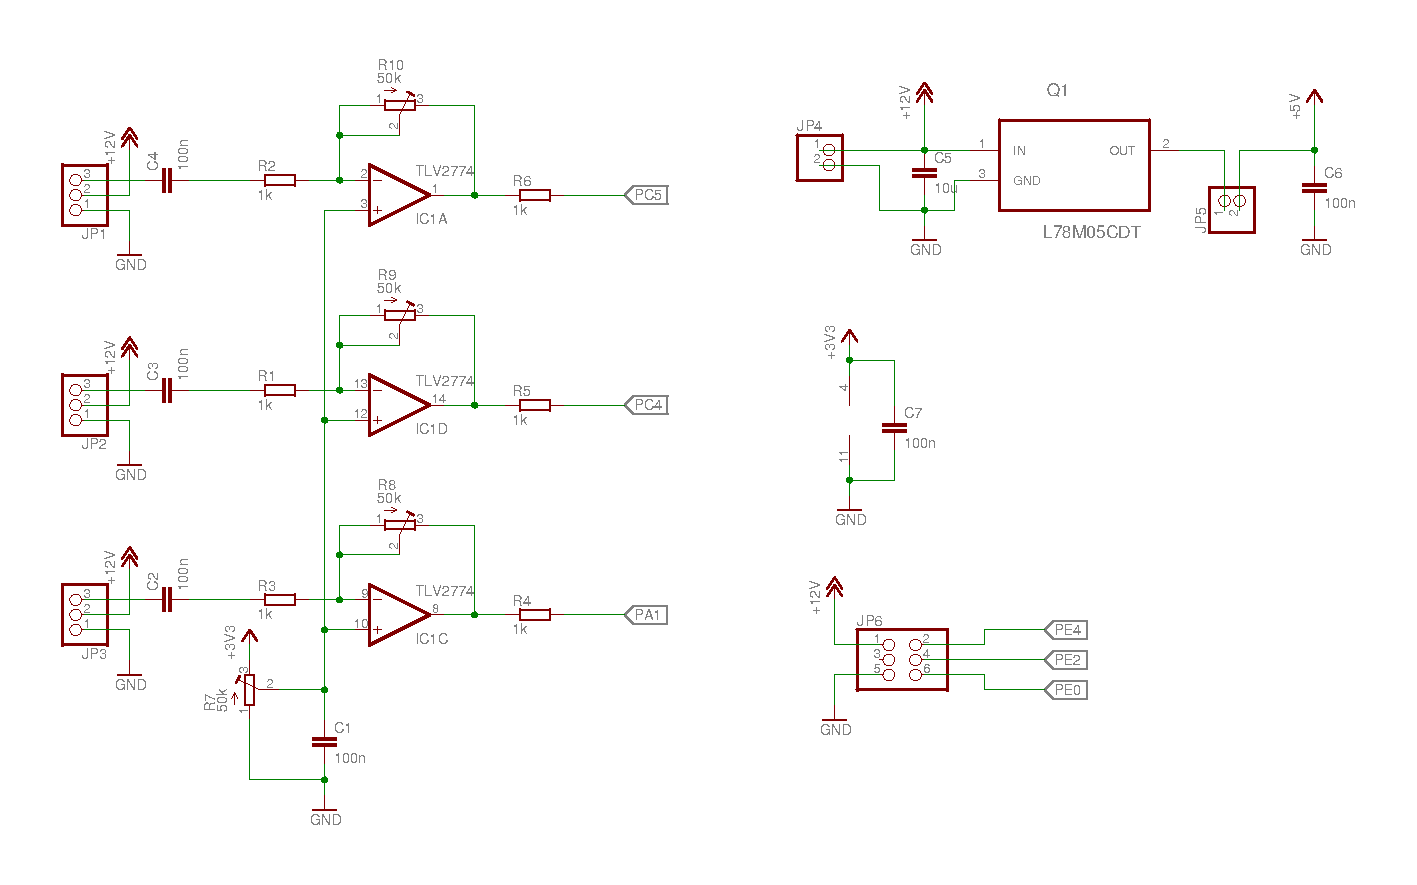
\includegraphics[width=1\textwidth, trim= 5mm 0mm 0mm 0mm,clip]{mainboard2}
    \caption{schemat przystawki do \textit{stm32f4-discovery}}
    \label{fig:przystawka}
\end{figure}


